\documentclass[conference]{IEEEtran}
\usepackage{stmaryrd}
\usepackage{amsfonts}
\usepackage{array, listings, color, todonotes, amsmath, algorithm}
\usepackage[noend]{algpseudocode}
\usepackage[bookmarks=false]{hyperref}

\usepackage{graphicx,times,amsmath} % Add all your packages here

\hyphenation{op-tical net-works semi-conduc-tor IEEEtran}

\lstset{ %
language=Java,                					% the language of the code
basicstyle=\ttfamily,       					% the size of the fonts that are used for the code
commentstyle=\color{lightgray},   
numbers=left,                   					% where to put the line-numbers
stepnumber=1,                   					% the step between two line-numbers. If it's 1, each line 
keywordstyle=\color{blue},
numbersep=5pt,                  				% how far the line-numbers are from the code
numberstyle=\color{lightgray},   
backgroundcolor=\color{lightestgray},  		% choose the background color. You must add
showspaces=false,               				% show spaces adding particular underscores
showstringspaces=false,        				% underline spaces within strings
showtabs=false,                 					% show tabs within strings adding
lineskip=-1pt,
tabsize=2,                      					% sets default tabsize to 2 spaces
captionpos=b,                   					% sets the caption-position to bottom
breaklines=true,                					% sets automatic line breaking
xleftmargin=10pt,
breakatwhitespace=false,        				% sets if automatic breaks should only
}

\newcommand{\code}[1]{{\lstinline!#1!}}

\IEEEoverridecommandlockouts    % to create the author's affliation portion
                % using \thanks

\textwidth 178mm    % <------ These are the adjustments we made 10/18/2005
\textheight 239mm   % You may or may not need to adjust these numbers again
\oddsidemargin -7mm
\evensidemargin -7mm
\topmargin -6mm
\columnsep 5mm

\begin{document}

\title{The 2013 Multi-objective Physical Travelling Salesman Problem Competition \thanks{Diego Perez, Spyridon Samothrakis and Simon Lucas are with the School of Computer Science and Electronic Engineering of the University of Essex (email: \{dperez, ssamot, sml\}@essex.ac.uk).} \thanks{Edward Powley, Daniel Whitehouse and Peter Cowling are with the Computer Science department of the University of York (email:  \{edward.powley, dw830, peter.cowling\}@york.ac.uk).} \thanks{This work was supported by EPSRC grant EP/H048588/1.}}

\author{Diego Perez, Edward Powley, Daniel Whitehouse, Spyridon Samothrakis, Simon Lucas, Peter Cowling}


% make the title area
\maketitle

\begin{abstract}
Numerous competitions have emerged in recent years... and this is another one.
\end{abstract}

% no key words

\section{Introduction}

\todo[inline]{Research in games and competitions.
Literature review.}~\cite{PerezCEC2012,MCTSSurvey}.

\section{The Multi-objective Travelling Salesman Problem}

The Multi-Objective Physical Travelling Salesman Problem (MO-PTSP) is a modification of the Physical Travelling Salesman Problem (PTSP), previously introduced by Perez et al.~\cite{PerezCEC2012} for the WCCI 2012 PTSP Competition. The PTSP is a game where the player controls a ship with the goal of visiting $10$ waypoints scattered around the maze in as little time as possible. MO-PTSP adds two more goals to the game: doing this spending as less fuel as possible and reducing the damage suffered by the ship. This section specifies the main components of the MO-PTSP game, such as the game physics, objectives, rules and maps. 

\subsection{Game Physics and the Real-Time Component}

Both PTSP and MO-PTSP are games that share some characteristics. One of these similarities is the physics of the ship used by the player to navigate through the game. In both games, the agent controls a ship where two different inputs can be applied: \texttt{steering} and \texttt{throttle}. The first input can be set to \textit{left}, \textit{straight} and \textit{right}, while the throttle input can be \textit{on} or \textit{off}. The combination of these inputs adds up to $6$ different actions that can be provided at a given time. Figure~\ref{fig:ship} depicts the moves available for the ship.

\begin{figure} [!h]
	\begin{center}
	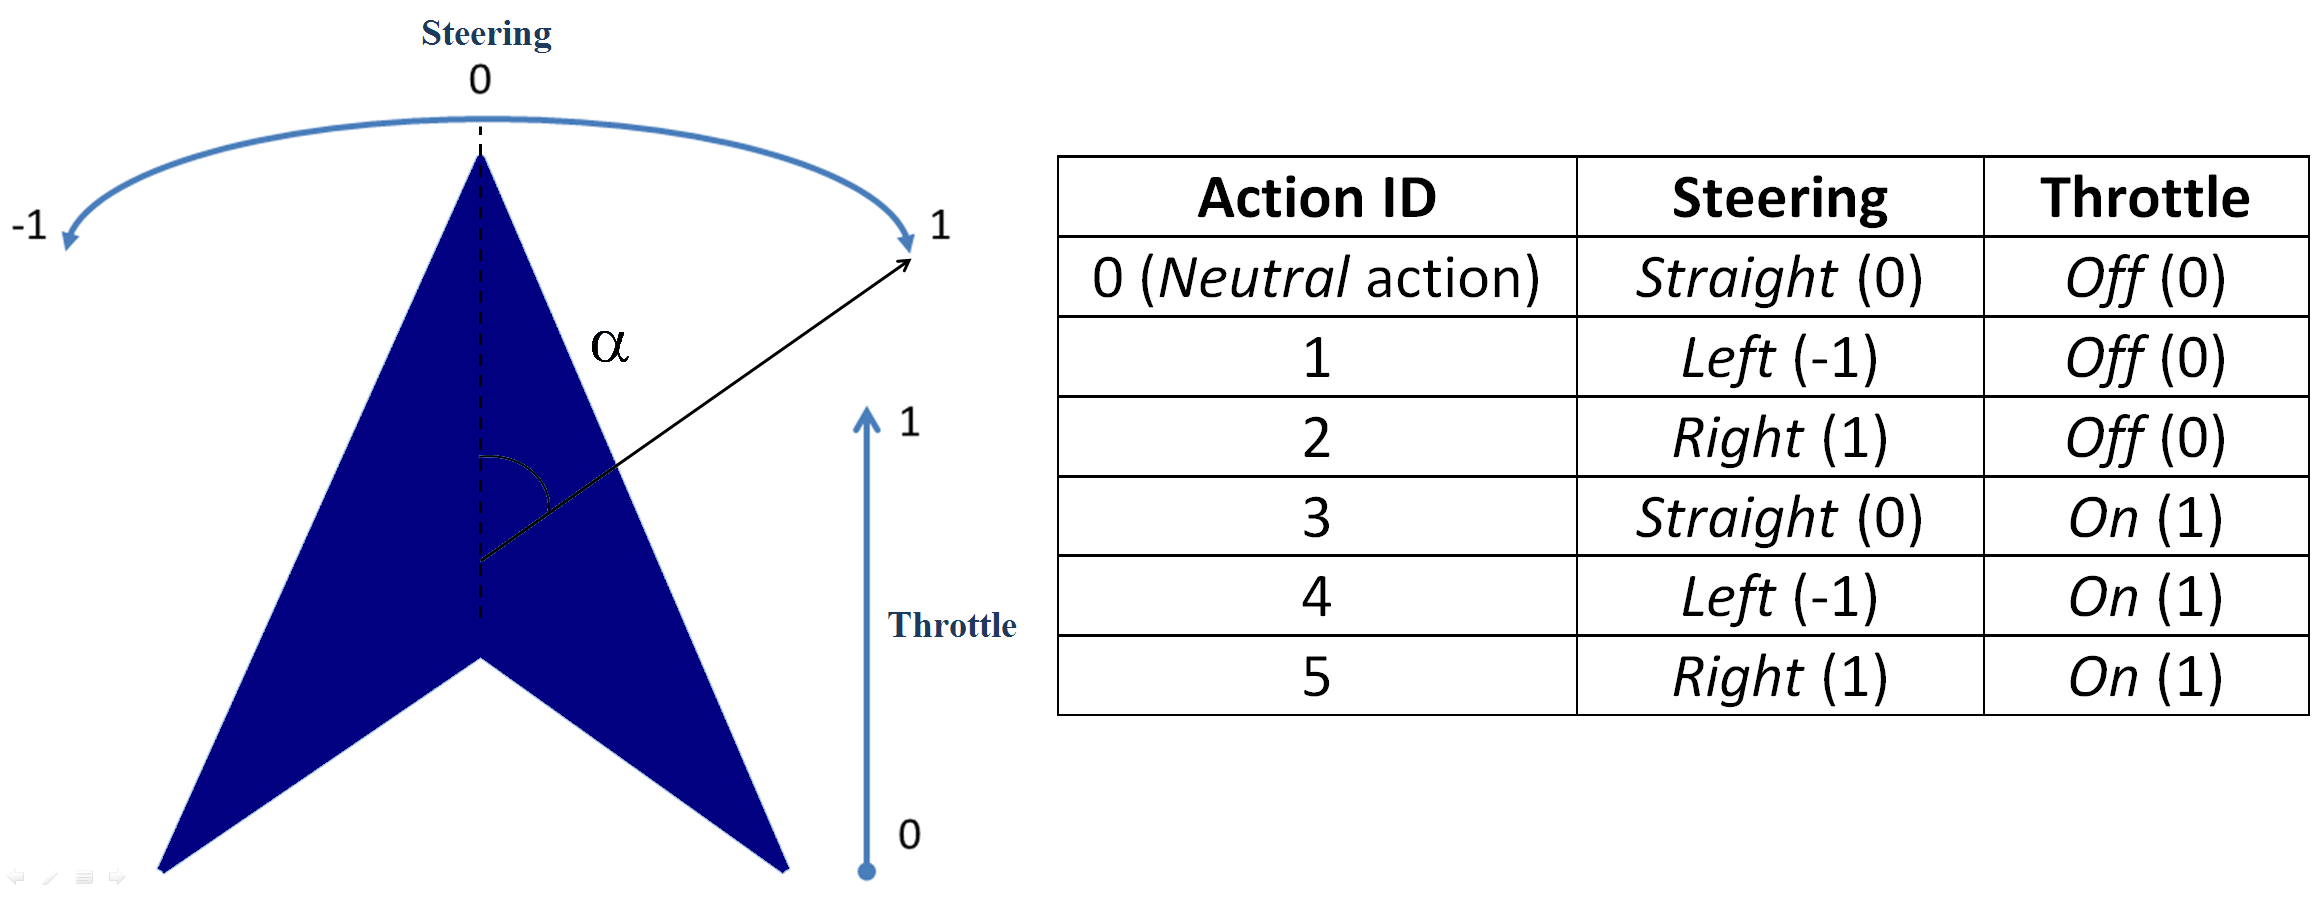
\includegraphics[scale=0.14]{img/ShipActions}
	\caption{Ship inputs and actions.}
	\label{fig:ship}
	\end{center}
\end{figure}

Left and right rotations are performed using a single angle, set to $\pi/60$ radians, and ship speed is set to $0.025$ pixels per time step, values determined by trial an error in order to provide a satisfactory game-play experience. The ship keeps its velocity from a game state to the next, making \textit{inertia} a key aspect to take into account when governing the ship. However, the ship would reach a full stop eventually if no acceleration actions are provided, as there is a loss of speed due to \textit{friction}. This friction is  set to $0.99$ (this is, only $1\%$ of the speed is lost at each step), a value also determined empirically. Finally, there is also a speed gain for actions with throttle on, which is set to $0.025$ pixels per game step. 

The location of the ship in the world can be uniquely determined by three vectors: \textit{position}, that specifies the coordinates of the center of the ship in the maze; \textit{direction}, a vector that indicates where the ship is pointing at (in other words, indicates the direction of a front vector); and \textit{velocity}, that determines the movement of the ship, including its direction and speed. Note that direction and velocity do not need to be aligned. Given an action, this part of state of the ship is modified as shown in Algorithm~\ref{alg:shipUpadte}.

\begin{algorithm}[!h]
\begin{algorithmic}
\Function{ShipUpdate}{$action$}
	\State $throttle \gets action.\Call{GetThrottle()}{}$
	\State $steering \gets action.\Call{GetSteering()}{}$

	\State $ship.direction.\Call{Rotates}{steering \times steerStep}$

	\If{$throttle == true$}
		\State $ship.velocity.\Call{Add}{ship.direction \times shipSpeed}$
	\EndIf

	\State $ship.velocity.\Call{Multiply}{frictionLoss}$
	\State $ship.position \gets ship.position + ship.velocity$


\EndFunction
\end{algorithmic}
\caption{Ship update function - no collisions.}
\label{alg:shipUpadte}
\end{algorithm}

The ship can also hit obstacles while it moves within the level, so position and velocity need to be updated differently if the ship's circular bounding collision hits a obstacle in the maze. When this happens, speed is reduced (by a $75\%$ factor) and the velocity vector is modified so the ship bounces off the wall with the appropriated angle. However, the MO-PTSP game introduces a new type of \textit{elastic} obstacle. In the case when the ship hits this kind of obstacle, the reduction of the speed is minor (only $10\%$), so the player can use this type of walls to change direction of travel abruptly without losing too much speed. A third type of obstacle (known as \textit{damaging} obstacle), produces a more important decrease in the speed of the ship, reducing it by a factor of $90\%$.

Another similarity between PTSP and MO-PTSP is the real-time component of the game: the player (also referred here as the agent, or the controller) must supply an action within a limited budget time, set to $40$ milliseconds. This limitation forces the controller to determine the next move quickly, rewarding those agents that are able to plan faster and explore the action search space in a more efficient manner.

While the PTSP was a bit more permissive, MO-PTSP imposes disqualifications in case this time limit is severely violated. In the original game, a neutral action was applied if the controller took more than $40$ milliseconds to provide an action, but no other consequences were derived from this misbehaviour. The game was then susceptible to cheating, as an agent could employ as long as it needs to plan ahead while the only consequence would be a neutral action in a single game tick. 

MO-PTSP tackles this situation by imposing a second time limit, set to $120$ milliseconds so, in case it is violated, produces the end of the game by disqualifying the player. Although controllers could still potentially spend more than $40$ milliseconds (with the same neutral move performed as a penalization), the risk of being disqualified and the limited gain that could be obtained by these extra milliseconds up to $120$ discouraged participants to performed this trick.

\subsection{A Multi-Objective Approach}

The main difference with respect to the original game, the PTSP, can be found in the three different objectives that need to be minimized:

\begin{itemize}
\item Time: the player must collect all waypoints scattered around the maze in as less time steps (or game cycles) as possible.
\item Fuel: the fuel consumed at the end of the game must be minimized.
\item Damage: the ship should end the game with as little damage as possible.
\end{itemize}

It is very important to stress that all waypoints must be visited in order to consider a game as successfully finished. Otherwise, a very simple but plausible approach for the player can be not to move at all and hence obtain a good result for the other two objectives (no fuel spent and damage suffered). A time dependant game over condition is established when the ship does not visit a waypoint once a timer has run off. This timer, initially set to $800$ time steps, is reduced by $1$ at every step if no waypoint is visited, causing the end of the game if it gets to $0$\footnote{PTSP also employed this timer, starting at $1000$. Hence, MO-PTSP is slightly more difficult in this sense, as it requires faster controllers.}. 

The ship starts with an initial fuel of $5000$ units, and one unit is spent every time an action with the throttle input set to \textit{on} is performed. The player adds, however, $50$ more units to the ship's fuel tank every time a waypoint is visited. Also, four \textit{fuel canisters} are also scattered around the maze, that provide $250$ units of fuel. It is important to mention that it is not mandatory to pick these fuel canisters up in order to complete the game, being their collection up to the strategy of the player. In case the amount of fuel available in the ship gets to $0$, the agent will not be able to use the throttle any more. 

Regarding the third objective, the ship can be damaged by two different game play elements. First, lava lakes are present in the game levels, dealing $1$ unit of damage for every game step the ship is flying over them. Secondly, the ship also gets damage when colliding with (non-elastic) obstacles, such normal and \textit{damaging} obstacles. The former type of obstacles (normal walls, also present in the PTSP game) inflict $10$ units of damage. The latter obstacles, created for this game, produce a more harming effect, dealing $30$ damage units. If the player's damage gets up to $5000$ units, the ship is destroyed and the game is over.

When the ship is damaged by a collision, it enters in an invulnerable state, where no more collision damage can be dealt to the agent (although lava still affects the ship) during $50$ game steps. This avoids situations when too much damage is suffered by the ship if it is touching an obstacle right after colliding with it.

\subsection{Game Maps}

Each level for the MO-PTSP game follows a specific format, based on the one that Nathan Sturtevant defined and was employed in several games such as Warcraft, Starcraft or Baldur's Gate. This type of maps have been used by some researchers in the literature before~\footnote{\url{http://movingai.com/benchmarks/dao/}}. The levels are stored in ASCII files, where each character determines the type of object or surface located at that pixel in the map grid. For MO-PTSP, these symbols are detailed next:

\begin{itemize}
\item Obstacles are represented by the characters 'T', 'D' and 'L', to be used to create normal, damaging and elastic obstacles respectively.
\item Normal surfaces use the character '.', while lava lakes employ ':'.
\item Waypoints and fuel canisters are indicated with 'C' and 'F' respectively.
\item The player's ship is represented by the character 'S'.
\end{itemize}

Figure~\ref{fig:sampleMap} presents an example of a MO-PTSP map, as it is drawn by the framework. Not visited waypoints are depicted as (filled) blue circles, while the already visited ones are shown as empty circles. Green ellipsis are used for the fuel canisters. Normal surface is brown, whereas lava is a red-dotted yellow surface. Elastic collisions are blue, normal collisions black and damaging collisions are drawn in red. The ship is drawn as a dark blue polygon, with a green triangle at the back denoting thrust being used. The trajectory followed by the ship is drawn with a black line.

\begin{figure} [!h]
	\begin{center}
	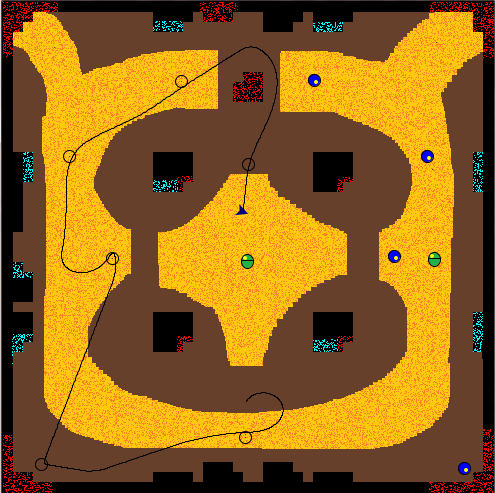
\includegraphics[scale=0.5]{img/sampleMap}
	\caption{Sample MO-PTSP map.}
	\label{fig:sampleMap}
	\end{center}
\end{figure}


\section{The MO-PTSP Framework}


\subsection{Software}

The MO-PTSP framework code can be downloaded from the competition webpage~\footnote{\url{http://www.ptsp-game.net/}}. The framework, under the name of \textit{Starter Kit}, contains the code, documentation, and 10 maps to test the controllers in. The software is written in Java, and it is organised in the following packages:

\begin{itemize}
\item Package \code{controllers}: this is the package where users can create controllers in. The framework already contains several sample controllers to help participants develop their own. Sample controllers are explained, and their performance studied, in section~\ref{ssec:sample}.
\item Package \code{framework}: it contains the main code of the game, and it is divided into several sub-packages:
\begin{itemize}
\item \code{core}: game entities, such as waypoints, fuel canisters, ship, etc. can be found in this package.
\item \code{graph}: this sub-package contains the code for a simple pathfinding tool, that can be used to calculate the shortest paths between any pair of points in the map (see Section~\ref{ssec:cont} for more details).
\item \code{utils}: several classes, useful for the framework such as 2D vectors and visual frames are included here.
\end{itemize}
\item Package \code{wox.serial}: this package contains a sample controller that uses the last version of the Wox Serializer~\footnote{\url{woxserializer.sourceforge.net}}. This is a useful implementation for controllers that use some kind of offline training, such evolutionary algorithms.
\end{itemize}

Additionally, the package \code{framework} contains three Java classes that allow the execution of the game:

\begin{itemize}
\item \code{ExecSync.java}: this is the main entry point of the framework. It allows the execution of the software in three different ways: running a controller in a given map, running it $m$ times in $n$ different maps, and starting the human player mode, where the game is played using the keyboard.
\item \code{ExecFromData.java}: allows the execution of the game in a map that has been initialized through data structures, instead of being read from a file. This mode can be employed for executions of large amount of consecutive runs, useful for reinforcement learning or evolutionary algorithms.
\item \code{ExecReplay.java}: every game played with the framework can have the actions performed by the controller saved into a file. This execution mode allows to replay a game previously saved from one of these files.
\end{itemize}

\subsection{Game flow}

In order to create a controller in this framework, a new class must be created that inherits from the base class \code{framework.core.Controller}. This class contains one abstract method which contains must be implemented: 

\begin{center}
\code{int getAction(Game, long);}
\end{center}

This method receives a copy of the current game state and a variable indicating when the controller is due to return with an action to execute. When the call to this method is done, this timer will be set to $40$ milliseconds later in time. The value returned by this method should be one of the following values, from \code{framework.core.Controller}, corresponding to the six actions available in the game:

\begin{itemize}
\item \code{ACTION_NO_FRONT}: Throttle off, no steering.
\item \code{ACTION_NO_LEFT}: Throttle off, steer left.
\item \code{ACTION_NO_RIGHT}: Throttle off, steer right.
\item \code{ACTION_THR_FRONT}: Throttle on, no steering. 
\item \code{ACTION_THR_LEFT}: Throttle on, steer left. 
\item \code{ACTION_THR_RIGHT}: Throttle on, steer right.
\end{itemize}

Apart from this method, every controller must implement a \code{public} constructor that receives the same two parameters: a game instance, with the initial state, and a time due. This constructor will be called just before the game starts, and allows the controller to initialize its own data structures and perform some initial planning. The budget time for the constructor of the controller is $1$ second, and the game will be over if this time is violated.

Hence, the game flow of MO-PTSP is simple: the framework creates the game, calculates the initialization due time ($1$ second from that instant) and class the controller's constructor to create the agent's object. If the constructor takes more time than the allowed, it is disqualified for this game. Then, until the game is over, the framework calls the function \code{getAction} to retrieve the next move to execute, providing the current game state and the time due for the calculation ($40$ seconds after the \code{getAction} call). In case this function takes more than $40$ milliseconds, the neutral action (\code{ACTION_NO_FRONT}) is executed. If the call took more than $120$ milliseconds, the game is over and the controller is disqualified for the game.

When the game is over, all actions executed by the agent can be dumped into a file. The format of this file will be the total amount of moves made, followed by each action returned, one per line.

\subsection{Game Interface} \label{ssec:cont}

Controllers can access information about the current state of the game using several functions available in the \code{Game} class. Agents can query the game about:

\begin{itemize}
\item Waypoints: location of the waypoints (both visited and yet to be collected), number of waypoints collected and how many are left to be visited.
\item Time: number of time steps since the beginning of the game, number of steps left to visit another waypoint.
\item Fuel: remaining fuel in the ship.
\item Damage: damage suffered so far in the game.
\item Fuel canisters: location of the canisters, both collected and not picked up yet.
\item Map locations: for every position in the map, identify the type of obstacle or surface in that location.
\item If the game is over or not.
\end{itemize}

A very important function that \code{Game} exposes to the controller is \code{tick(int action)}. This method advances the game state by applying the action indicated as a parameter. By using this function, the agent can foresee the effects in the game of the actions performed, allowing to perform planning in a closed loop manner. 

The framework also comes with a simple implementation of path-finding using the A* algorithm. A 8-way connected graph is created in the navigable parts of the map, given a certain granularity (separation between the graph's nodes). This graph is only created if the agents wants to use it, so the computational time it takes is not detrimental to those participants who do not want to use it, or prefer to work on a more sophisticated/efficient path-finding implementation for the game.

\section{The MO-PTSP Competition}

\subsection{Controllers for the competition}

The controllers submitted for the competition must run in the framework provided within the \textit{Starter Kit} and, in order to be a valid controller, the following characteristics must be observed:

\begin{itemize}
\item Multi-threading is not allowed.
\item During execution, it is possible to read from files, although writing is only allowed if this is done in the controller's own directory.
\item The process that runs the agent must not use more than 256MB of memory.
\item It must be written in Java. Participants must submit the source code in a zipped file, and the competition server will unzip, compile and run the controller in the appropriate set of maps. The controller must be submitted before the competition deadline, and a short description of the technique employed is expected.
\end{itemize}


\subsection{Ranking entries}

One of the main challenges of a multi-objective competition is to evaluate and rank entries according to its performance. In a single objective scenario, this is straightforward: if the objective of the game is to maximize a score, or minimize completion time (like in the original PTSP), the best result will be the one with the maximum or minimum value measured.

However, multi-objective games pose the problem of evaluating objectives that could be in conflict (and are in this particular case). A clear example is the opposed objectives of time and fuel: minimizing completion time would naturally be achieved with a higher speed, which is done by pressing the throttle more often and therefore spending more fuel. In a similar way, very fast controllers  would usually follow straight line distances, but this will most of the time make the ship drive through lava lakes, increasing the damage taken.

The competition states that none of these objectives should be preferred over the others. In other words, all these three objectives must be optimized simultaneously. In order to evaluate entries that run in a single map, the competition uses concepts borrowed from \textit{Pareto optimality}. Given a single map, where $n$ results from different competitors have been obtained, the entries are ranked in \textit{Pareto fronts}.

A MO-PTSP solution can be seen as a triplet $S = <T, F, D>$, where $T$ is the time taken to complete the game, $F$ is the fuel spent and $D$ is the damage taken by the ship at the end of the run. Applying concepts of Multi-Objective optimization, it is said that a solution $S_1$ \textit{dominates} another solution $S_2$ (and it is written $S_1 \preceq S_2$) if:

\begin{enumerate}
\item $S_1$ is no worse than $S_2$ in all three objectives.
\item At least one objective in $S_1$ is strictly better than its analogous counterpart in $S_2$.
\end{enumerate}

Dominance provides a partial order in the solutions provided. However, there are some cases where it is not possible to say that $S_1$ dominates $S_2$ or vice versa (an example in MO-PTSP would be when $S_1$ is better in the time objective, but $S_2$ spends a smaller amount of fuel than $S_1$). When this happens, it is said that these two solutions belong to the same Pareto front. If there is no solution found that dominates a given solution $S$, then $S$ belongs to the \textit{optimal Pareto front}.

Thus, it is possible to rank all entries in a single map in different Pareto fronts, and there will always be an optimal front with results no better than those allocated to that front. Once the results have been sorted in fronts, points are given to the entries using the following scheme:

\begin{itemize}
\item Only the entries that placed a result in the optimal Pareto front are awarded with points. All other results obtain $0$ points in this map.
\item $1$ point is awarded to the entry that was able to place a result in the optimal Pareto front.
\item The best result for each objective is tracked, and points are awarded to the entries that achieved these records. $2$, $9$ and $24$ additional points are awarded to the entries that obtained respectively $1$, $2$ and $3$ records in a single execution in a map.
\end{itemize}

This scheme of points rewards those entries that dominate clearly other contestants. For instance, if one result is better than all others in all objectives, it will be the only member of the optimal Pareto front and it would receive a total of $25$ ($24 + 1$) points in that map, as it obtained the best result in all objectives.

A more common scenario is shown in Table~\ref{tab:rankingSample}, taken from the final rankings of the competition in one of the starter kit maps. The first three entries receive $1$ point as they are in the optimal pareto front, whereas the last two (dominated by at least one of the first three entries) receive no points. The first one obtains the best result in time and damage, so it gets $9$ extra points. The second entry gets the best result in fuel, being rewarded with extra $2$ points. Finally, the third entry only receives $1$ point as it doesn't achieve any record in this map, but it is still in the optimal front because no other entry dominates it.

\begin{table}[!t]
\begin{center}
\begin{tabular}{|>{\centering\arraybackslash}m{1.25cm}|>{\centering\arraybackslash}m{1.15cm}|c|c|>{\centering\arraybackslash}m{0.9cm}|>{\centering\arraybackslash}m{1.5cm}|}
\hline
 \textbf{User} & \textbf{Waypoints} & \textbf{Time} & \textbf{Fuel} & \textbf{Damage} & \textbf{Points} \\ 
\hline
PurofMovio & $10$ & \textbf{1745} & $403$ & \textbf{301} & $9 (+1) = 10$\\
\hline
mmorenosi & $10$ & $4472$ & \textbf{182} & $812$ & $2 (+1) = 3$\\
\hline
epowley & $10$ & $2737$ & $227$ & $519$ & $0 (+1) = 1$\\
\hline
\hline
macrors & $10$ & $1747$ & $761$ & $393$ & $0$\\
\hline
Weijia & $10$ & $1809$ & $590$ & $485$ & $0$\\
\hline
\end{tabular}
\caption{Example of entries ranked in a single map. }
\label{tab:rankingSample}
\end{center}
\end{table}

Another important aspect to determine is how many runs a controller performs in a given map. On one hand, only a single run (also referred here as a \textit{match}) would penalize those unlucky cases where the controller behaved poorly, or even did not visit all waypoints. On the other hand, running several matches and calculating the average for each objective would provide misleading results (a controller could try to optimize only one objective per run, and the average would show results that do not match with the real behaviour in a single match.

The approach taken in this competition is the following. Each controller is allowed to run a maximum of $5$ times on each map, but the evaluation stops as soon as one match visits all waypoints. Then, the result of that particular run is used to rank the entry.

Finally, when a controller is evaluated in a set of $n$ maps, the final score is the sum of the points awarded on each one of these levels. To compute the rankings in a set of maps, the entries are sorted according to this total amount of points, and the one with the highest score is declared the winner.
	
	
\subsection{Competition Rankings}

The MO-PTSP Competition is composed of three different tracks, all of them running in parallel.

\subsubsection{Bot Competition Track} This track evaluates controllers (bots) submitted to the competition. Before the deadline of the competition, some preliminary rankings are computed in the contest server. Every time a participant submits a controller, it is evaluated on a set of $20$ maps, and the rankings of this set are automatically updated in the website. This allows participants to compare between themselves, and get a feeling about how well their controllers would perform for the final rankings.

The set of maps is renewed every few weeks, in order to avoid the controllers to overfit to any particular set. All these maps are taken from a pool of unknown maps, that does not include the levels from the starter kit. The final evaluation, after the deadline of the competition, is run in a new set of maps, where some are taken from the previous sets and others are completely new to the participants.

\subsubsection{Human Competition Track} The website allows players to register and play ``as humans'' the $10$ games from the framework starter kit in an applet. These games are saved and rankings are drawn to determine the best MO-PTSP human player.

\subsubsection{Human vs. Bot Competition Track} Every time a controller is submitted to the bot competition track, it is also executed in the starter kit maps. Then, a separated ranking is calculated between the results obtained by the bots and the humans in these maps, allowing a direct comparison between bots and humans in the MO-PTSP game.

\subsection{Sample Controllers} \label{ssec:sample} 

\todo[inline]{Sample controllers: random, greedy, macro-action random search controller. Include some measurements.}

\section{Results of the competition}

\todo[inline]{Describe results in detail.}

\section{The winning entry}

This section gives a high-level overview of the winning entry, \textsc{PurofMovio}.
Further details can be found in~\cite{Powley2013_moptsp}.
\textsc{PurofMovio} is based on \textsc{Purofvio}, the winning entry to the previous (single-objective) PTSP competitions~\cite{Powley2012,Perez2013}.

\subsection{Architecture}

The controller has three main components.

\subsubsection{Distance mapper}
During controller initialisation, the shortest-path distance between every waypoint and every other pixel on the map is computed
using a scanline flood fill algorithm~\cite{Lieberman1978}.
This means that during controller execution
the distance of a future ship position from the next waypoint can be queried rapidly.
The distance mapper takes lava into account when computing distances:
moving across a pixel of lava costs the same as moving across $1+\gamma$ pixels of empty space,
where $\gamma$ is a tunable parameter.
An example of a distance map is shown in Figure~\ref{fig:distance-map-weighted}.

\begin{figure}%
\begin{center}
	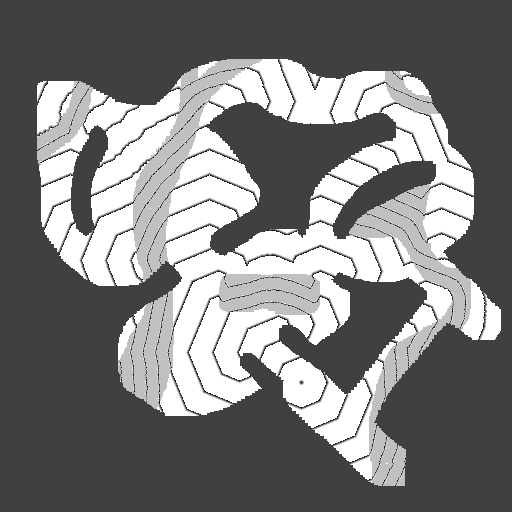
\includegraphics[width=0.8\columnwidth]{img/distance-map-weighted.png}%
\end{center}
\caption{An example of a distance map with a lava weighting of $\gamma = 1$. The contour lines correspond to distances a multiple of $25$ pixels from the origin (shown as a dot).}%
\label{fig:distance-map-weighted}%
\end{figure}

\subsubsection{Route planner}
Also during controller initialisation, the order in which to visit the waypoints is determined.
Fuel tanks are also included as ``optional'' waypoints.
The route planner uses classical TSP methods, namely the multiple fragment heuristic~\cite{Bentley1990} and 3-opt local search with first improvement~\cite{Lin1965,Johnson1997}.
The edge weights in the TSP graph are the shortest-path distances calculated by the distance mapper.

3-opt is a hill-climbing algorithm.
Starting from an initial path,
it considers all triples of edges in the path
and all ways in which the path can be reconnected when those edges are deleted.
If a resulting path has a lower cost than the initial path,
the new path is kept and the process begins again.
This continues until no further improvements can be made.
In the classical TSP the cost of a path is its length, i.e. the sum of the weights of its constituent edges.
In \textsc{PurofMovio} the cost measure is modified to take the physics of MO-PTSP into account:
paths which require sharp turns at waypoints or indirect paths between waypoints incur cost penalties.

\subsubsection{Ship controller}
During controller execution,
the ship is controlled by Monte Carlo Tree Search (MCTS)~\cite{MCTSSurvey}
with several modifications to deal with the real-time aspect of the problem.
Instead of choosing a potentially different action on every time step,
the controller instead chooses a \emph{macro-action},
an action to be repeated for the next $T$ time steps.
This means that instead of having $40$ milliseconds to choose each action,
the controller has $40T$ milliseconds to choose each macro-action.
This reduces the controller's ability to make fine-grained adjustments to the ship,
but is a worthwhile tradeoff.

The second modification deals with the length of the game,
which even with macro-actions can result in a decision tree several hundred plies deep.
We impose a fixed horizon on MCTS. After $d$ plies,
all states are treated as terminal: children are not expanded, simulations are halted.
The resulting nonterminal state is evaluated by a heuristic evaluation function.
The most crucial terms in the evaluation function are the number of waypoints collected so far, and the distance from the ship to the next waypoint in the route.
There are also evaluation terms for fuel and damage, with tunable parameters to control the emphasis placed on these objectives.

\begin{figure}%
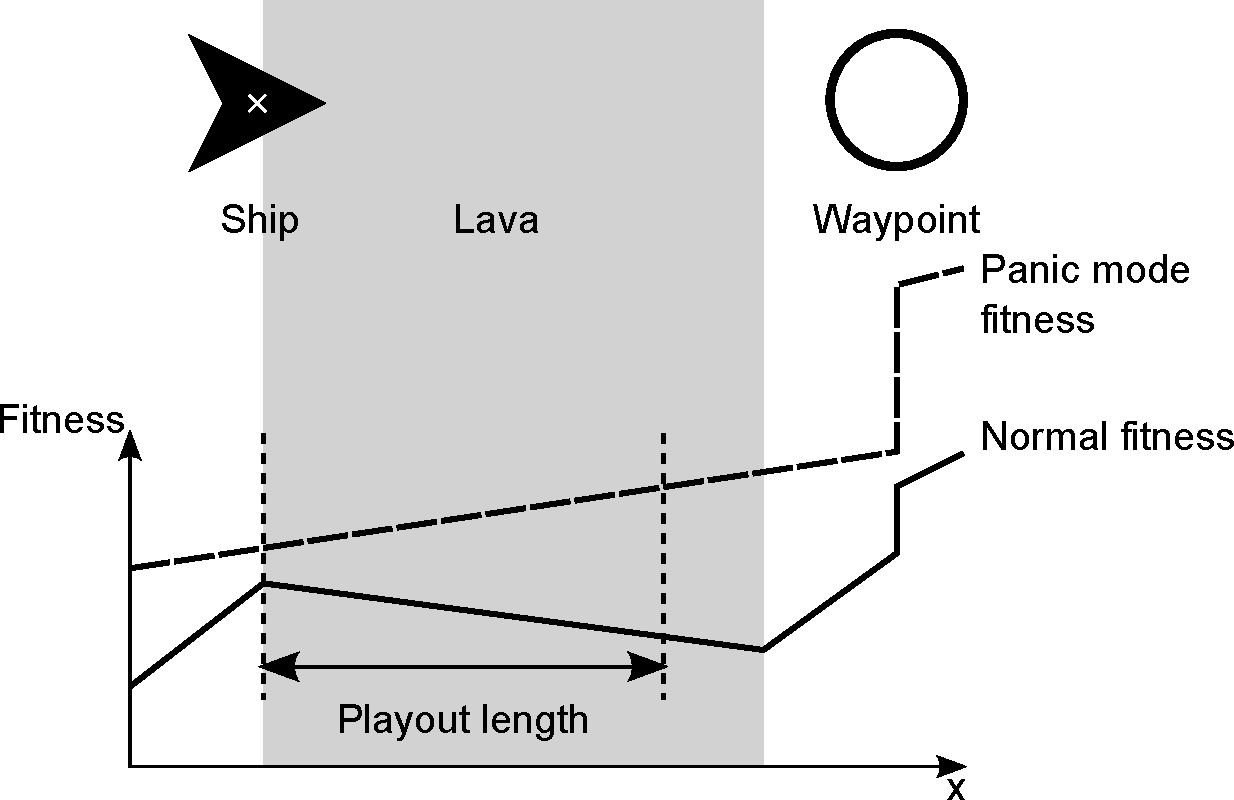
\includegraphics[width=\columnwidth]{img/local-optimum.pdf}%
\caption{Illustration of a low quality local optimum in a simplified \mbox{$1$-dimensional} version of MO-PTSP.}%
\label{fig:local-optimum}%
\end{figure}

The controller may sometimes become trapped in a local optimum,
where the search horizon is too short to see a path towards the next waypoint.
An example of this is shown in Figure~\ref{fig:local-optimum}.
The fitness function gives a reward for approaching the next waypoint but a penalty for damage incurred by driving through lava.
The playout length is insufficient for the search to determine that driving through the lava eventually leads to the next waypoint and thus a higher fitness,
so the controller instead decides to sit at the edge of the lava until the game times out.
We introduced a mechanism called \emph{panic mode} to deal with this:
if it is detected that MCTS is failing to find lines of play that make progress towards the goal,
the search switches to an alternative evaluation function which more aggressively guides the controller towards the next waypoint (ignoring fuel and damage).
The original evaluation takes over again once the controller is unstuck from the local optimum.
We found that panic mode has a limited impact on the time, fuel and damage scores of the controller,
but improves its ability to collect all waypoints without timing out.

\subsection{Parameter tuning}

\textsc{PurofMovio} has $18$ tunable parameters in total.
We found hand-tuning of the parameters to be challenging:
small changes in parameter values can have large and unpredictable effects on the behaviour of the controller,
and the randomised nature of MCTS makes it difficult to assess whether an observed change in behaviour is due to a recent parameter change
or simply a lucky or unlucky run.

The parameters were tuned using the \emph{Covariance Matrix Adaptation Evolution Strategy (CMA-ES)} algorithm~\cite{Hansen2001}.
CMA-ES optimises a vector of real-valued parameters by repeating three steps:
first, a population is sampled at random according to a multivariate normal distribution;
second, the population is sorted in order of fitness;
third, the fittest individuals are used to skew the distribution used for subsequent samples.
As these three steps are repeated, the sampling distribution converges on an optimum.

Since CMA-ES does not use scalar fitness values but only the fitness ranking of the population,
it is readily adapted to multiobjective problems~\cite{Igel2007}.
To measure the fitness of a particular parameter vector,
the controller is executed once on each of the $10$ starter kit maps and the total time, fuel and damage are measured.
The population is then ranked by \emph{non-dominated sorting}:
individuals on the Pareto front receive rank~$1$ and are removed;
from what remains of the population, individuals on the new Pareto front receive rank~$2$ and are removed;
and so on until the population is exhausted.
Within each rank, the individuals are sorted by the sum of time, fuel and damage, with equal weights.
Igel et al~\cite{Igel2007} suggest more sophisticated tie-breaking schemes, but due to time constraints we chose not to implement these.

Results of parameter tuning are presented in~\cite{Powley2013_moptsp}.
We ran the parameter tuning three times, obtaining three different sets of parameters.
The three tuned controllers outperform our best efforts at hand-tuning,
but make slightly different tradeoffs between the three objectives:
for example the third set performs worse on time than the other two, but uses significantly less fuel.

CMA-ES is able to handle noisy and esoteric fitness landscapes, and is explicitly designed not to require tuning.
This makes it especially attractive as a ``black box'' optimisation method;
the mathematics behind it is sophisticated but can largely be ignored by the user.
A mature Java implementation has been made freely available by the algorithm's creators\footnote{\url{https://www.lri.fr/~hansen/}},
and this implementation was used to tune the parameters for \textsc{PurofMovio}.

\section{Conclusions}

\todo[inline]{We had lots of fun.}

\bibliographystyle{IEEEtran}
\bibliography{IEEEabrv,biblio}

\end{document}
